\documentclass[thesis]{subfiles}

\begin{document}

\OnlyInSubfile{\setcounter{chapter}{5}}

\chapter{Implementation of molecular simulation software}

Part of my PhD project was to work on the implementation of molecular simulation
software as part of the Domino software library. In this chapter, I will describe
the context of this project and my contributions to it, as well as some advanced
simulation techniques I worked to incorporate in Domino. The first of these
advanced methods is the Hybrid Monte Carlo simulation technique, which joins
molecular dynamics and Monte Carlo to exploit the advantages of both. I will
present the original method and some of the most recent developments and
improvements to it. I also explored methods for dealing with the treatment of
electrostatic interactions in the context of periodic boundary conditions. I
will first describe the Ewald summation technique, and some tricks for
optimizing its implementation in the Domino code base. Then I will discuss the
Wolf summation method as a possible alternative to Ewald summation that only
relies on a sum of pairwise terms.

\newpage
\section{Domino: extensible molecular simulations library}

Domino is a \cxx library designed for classical atomistic molecular simulations.
In this section, I will present its design, the code base and my contributions
to it, as well as some of the project goals and software architecture choices
made to reach these goals.

Domino is written in \cxx, a computer programming language created in 1983 by
Bjarne Stroustrup as an extension of the C language. \cxx mainly adds
object-oriented programming, functions overloading and generic programming to C.
We chose \cxx because it is a general-purpose language, which we can use to
implement complex algorithms while retaining the ability to manage memory
allocations, locality, and layout. These two last points are what allows \cxx to
run faster than \emph{managed} languages, where the users don't have explicit
control over memory management. Using \cxx does not necessarily makes software
faster, but it enables developers to optimize the code more than other
languages. Domino uses the \cxx11 version of \cxx standard, which brought major
changes to the language, making it easier to use correctly and more expressive.

In this section, I will assume some basic programming, \cxx and object-oriented
knowledge from the readers. There are a lot of great online resources on all of
these subjects, as well as books such as \emph{\cxx Primer}\cite{Lippman2012},
or \emph{Effective Modern \cxx}\cite{Meyers2014}. Concerning the algorithms I
implemented, I found the book by Frenkel and Smit\cite{Frenkel2002} to be a
great help.

\subsection{Goals and architecture}

The main goal of Domino is to be an extensible classical molecular simulation
library. A software library is a collection of functions and classes working
together to provide a given functionality. One specificity of Domino is that it
provides facilities to run both classical Monte Carlo, molecular dynamics and
energy minimization simulations, where most other simulation software only offer
either Monte Carlo or molecular dynamics as \emph{first-class citizen}. Notable
exceptions that provide both Monte Carlo and molecular dynamics include
RASPA\cite{Dubbeldam2015} and Sire\cite{SireMol} software. We also try to make
Domino easy to use, and easy to extend, meaning it can be used as a basis for
the development of new molecular simulations methods. These goals translate into
some of the architectural choices: in particular, the code needs to be simple to
understand in order to be simple to extend. This means I restricted myself to a
simple subset of \cxx, not using complex template-based meta-programming or deep
class hierarchies.

The behavior and capabilities of Domino can be extended using two different
mechanisms. Classes that provide central behavior, such as potentials or
molecular dynamics integrators are manipulated through pointers to the
corresponding pure virtual base class --- or \emph{interface} --- throughout the
code. By creating a new class inheriting from this interface, it is possible to
add behavior to Domino without having to modify any of its internal source code.
For example, the source code listing~\ref{code:potential} shows the interface
used for potentials and the implementation for Lennard-Jones potentials. Adding
a new potential to Domino is as simple as creating a new class and implementing
the corresponding required functions: \texttt{energy} and \texttt{force}. Other
extensible parts of Domino include Monte Carlo moves, molecular dynamics
thermostat and integrators, and simulation propagators.

\newpage
\begin{listing}[ht]
    \begin{minted}[autogobble, fontsize=\small]{c++}
    /// Abstract base class for all energy and forces computations. All
    /// functions take an abstract parameter 'x' that will be the distance for
    /// pair potentials and the angle for angles or dihedral angles potentials.
    class Potential {
    public:
        Potential() = default;
        virtual ~Potential() = default;

        /// Get the energy for the parameter `x`
        virtual double energy(double x) const = 0;
        /// Get the force factor for the parameter `x`
        virtual double force(double x) const = 0;
    };

    class LennardJones final: public Potential {
    public:
        LennardJones(double epsilon, double sigma): sigma_(sigma), epsilon_(epsilon) {}

        double energy(double r) const override {
            auto sr = sigma_ / r;
            auto sr3 = sr * sr * sr;
            auto sr6 = sr3 * sr3;
            return 4 * epsilon_ * sr6 * (sr6 - 1);
        }

        double force(double r) const override {
            auto sr = sigma_ / r;
            auto sr3 = sr * sr * sr;
            auto sr6 = sr3 * sr3;
            return -24 * epsilon_ * sr6 * (1 - 2 * sr6) / r;
        }

    private:
        double sigma_ = 0;
        double epsilon_ = 0;
    };
    \end{minted}
    \caption{Extract of the definition of the \texttt{Potential} interface in
    Domino, and implementation for Lennard-Jones potential.}
    \label{code:potential}
\end{listing}

The other way it is possible to extend Domino is by adding directly adding code
before, inside or after the simulation loop. As a library, Domino does not
impose a structure on the simulation program. It is thus possible to customize
the simulation flow, adding \emph{on-the-fly} analysis, or merging multiple
molecular dynamics simulation into a parallel tempering one. See the source code
listing~\ref{code:simulation-example} for a simple example of constant pressure
Monte Carlo simulation, showing how a simple simulation can be created by
calling the high-level functions of the Domino library.

\begin{listing}[ht]
    \begin{minted}[autogobble, fontsize=\small]{c++}
    #include "domino.hpp"
    using namespace domino;

    int main(int argc, char *argv[]) {
        domino::initialization();

        // Read the system
        auto system = Trajectory("initial.pdb").read();
        // Read the interaction potential
        domino::InputFile("potential.yml").read_to(system);

        // Setup the simulation: Monte Carlo at 300 K with three moves
        auto mc = MonteCarlo(units::from(300, "K"));
        mc.add_move(Translate(units::from(0.5, "A"), 50));
        mc.add_move(Rotate(units::from(20, "deg"), 50));
        mc.add_move(Resize(units::from(500, "bar"), 1));
        mc.setup(system);

        // Add code before the simulation loop
        // ...

        // Simulation loop
        for (size_t i=0; i<1e6; i++) {
            // This function call will propagate the simulation for one step
            mc.propagate(system);

            // Add code inside the simulation loop
            if (i % 100 == 0) {
                std::cout << i << " " << system.energy() << "\n";
            }
        }

        // Add code after the loop
        std::cout << mc.summary() << std::endl;

        domino::finalization();
        return 0;
    }
    \end{minted}
    \caption{Example of a constant pressure Monte Carlo simulation using Domino.}
    \label{code:simulation-example}
\end{listing}

\newpage
\subsubsection{Contributions to Domino}

The Domino project was started in 2009 by François-Xavier Coudert and Anne
Boutin. Before I started working on it in 2015, it had contributions by
Jean-Marie Teuler, Julien Germond and David Bousquet. Since then, I have been
the sole contributor to the code, and rewrote most of it, creating 480 git
commits (self-contained modifications) out of the 800 of the repository. My
contributions were related to two principal areas of the code: code quality
improvement and simulation algorithms implementation.

On the code quality improvements side, I ported Domino to \cxx11, and cleaned up
multiple previous experiments, such as a Python binding, atomic selection
language and file input and output (for which I developed the standalone
chemfiles library, presented in appendix~\ref{sec:chemfiles}). I added tests
with respect to NIST simulation reference data\cite{NIST}, as well as an input
file system to specify interaction potentials. I improved the simulated system
in-memory representation and canonicalization: dealing with normalization of
bond and angles indices and representation of the bonded distance matrix.

On the side of algorithms implementation, I added the interface-based
extensibility of Domino. I also implemented grand canonical and hybrid Monte
Carlo moves, as well as an anisotropic Berendsen barostat, a Monte Carlo
barostat and the CSVR thermostat for molecular dynamics. I improved the support
for anisotropic simulations by implementing anisotropic stress and pressure
calculations for both Monte Carlo and molecular dynamics. I implemented both
Ewald and Wolf summation methods for electrostatic energy and forces
calculations. Finally, I improved the caching of energy in Monte Carlo
simulations, adding support for more types of move and electrostatic
interactions.

\subsection{Challenges encountered}

I encountered a few challenges while working on Domino, some of which are
generic to the field of molecular simulation, others which were specific to the
fact that Domino provides both Monte Carlo and molecular dynamics. I will
present here some of these challenges, as well as the technical solutions I
developed to overcome them. Several of these challenges were related to the
efficiency of computing the energy and forces under periodic boundary
conditions, which are the most expensive steps of simulations.

\subsubsection{A performance model of modern computers}
\label{sec:computer-model}

\begin{figure}[b]
    \centering
    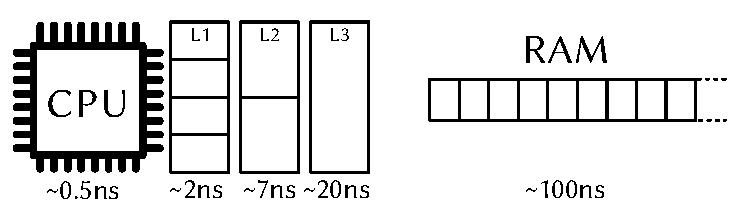
\includegraphics[width=0.7\textwidth]{figures/images/computer-model}
    \caption{Latency for data access from the CPU to three level of CPU cache
    (L1, L2 and L3) and the RAM of a modern computer. The numbers are for Intel
    Corporation's i7 and Xeon CPUs\cite{SO-CPU-latency}.}
    \label{fig:computer-model}
\end{figure}

At their basis, computers are made of two main components: the central
processing unit (CPU) or processor executes the instructions, and the memory ---
usually in the form of random access memory (RAM) --- stores data used by the
processor. On the first personal computers in the 80s, CPU executed instructions
at \SI{1}{MHz}, and RAM accesses were made at roughly the same speed. Optimizing
code then mainly meant reducing the number of instructions executed by the CPU.
Since then, CPU speed increased dramatically to around \SI{4}{GHz}, while the
RAM access speed only increased to \SI{10}{MHz}. This means that data access
patterns are much more important to consider when optimizing software for low
run time. In order to speed up data access, modern CPUs come with multiple
levels of cache, from the fast but small first level (L1) cache, to the bigger
but slower L2 and L3 caches. Upon the first access, data is copied from RAM to
the cache, and on subsequent read or write operations, the data from the cache
is used. Later on, data is copied back to RAM. Typically latency for data access
on caches and RAM are represented on figure~\ref{fig:computer-model}.

Because the CPU can spend hundred of cycles waiting for data which is not yet in
the caches, it is important to make sure data in the RAM is accessed in a predictible
way. When some data is explicit fetched from the RAM, another mechanism
called \emph{pre-fetching} kicks in, fetching additional data close to the one
requested and storing it in the cache. If the code accesses data in a linear
way, the next data fetch will be faster, as everything required is already in
the caches. Software behaving this way is said to have high \emph{memory
locality}. Improving memory locality is nowadays an additional important part of
software optimization.

\subsubsection{Mixed molecular dynamics and Monte Carlo}

Monte Carlo, and in particular Grand Canonical Monte Carlo, requires a different
set of operations on the system that molecular dynamics, and has a different
optimal data representation. Specifically, Grand Canonical Monte Carlo requires
the possibility to dynamically change the number of molecules, and prevents the
use of atomic index as atomic identifiers, as the indices will change during the
simulation. At the same time, molecular dynamics can benefit from distributed
memory parallelism (using for example the \emph{Message Passing Interface} MPI)
by using a domain decomposition algorithm, but this kind of parallelism is less
trivial to integrate efficiently with Monte Carlo. To both allow GCMC
simulations and future implementation of distributed memory parallelism for
molecular dynamics, the storage of atoms (and the associated properties) uses
dynamic allocation in growable containers. Furthermore, atoms from the same
molecules are kept contiguous in memory, improving memory locality when
computing intra-molecular interactions and allowing the implementation of domain
decomposition.

Moreover, molecular dynamics needs information on the forces acting on the
system, while Monte Carlo only needs to compute the energy. When computing the
forces, adding the energy is a minimal additional runtime cost --- periodic
boundary conditions have already been applied --- and no additional memory cost.
On the opposite, when computing energy, adding forces increases both the memory
and runtime cost: for a small system containing 50 water molecules, computing
only the energy with Domino takes \SI{1.3}{ms}, and computing the energy and the
forces takes \SI{2.6}{ms}. Domino thus provides two different code paths, one
computing only the energy for Monte Carlo and another one computing both the
energy and the forces for molecular dynamics.

\begin{figure}[ht]
    \centering
    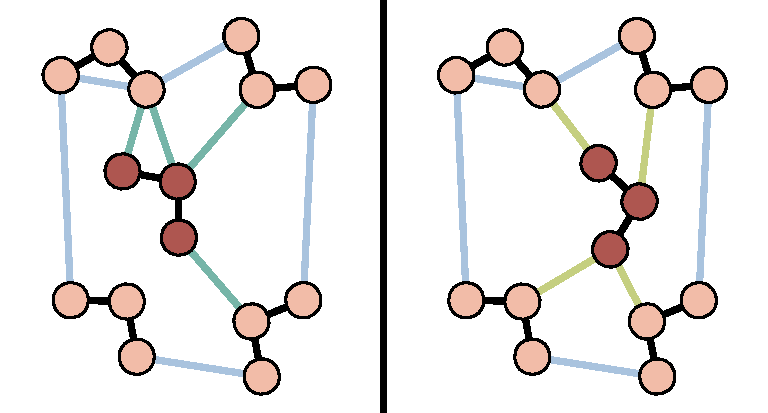
\includegraphics[width=.7\textwidth]{figures/images/mc-cache}
    \caption{Illustration of the use of an energy cache with Monte Carlo
    simulation. Before the move, all the interaction contributions are computed
    and stored. After the move, only the interactions in green needs to be
    computed to get the energy difference. Not all pair contributions are
    represented on the figure.}
    \label{fig:mc-cache}
\end{figure}

Another possible improvement to the speed of simulations comes from the fact
that most Monte Carlo moves only update the positions of a few atoms. This
means that most of the energy components do not change before and after the
move. Instead of recomputing all the energy components when evaluating the
energy difference $\Delta U$ in the Metropolis criterion, Domino uses a cache
for the energies, storing the energy associated with a pair in a bi-dimensional
array, and only updating the energies associated with the modified pairs. This
strategy is illustrated in figure~\ref{fig:mc-cache}. This can result in
multiple orders of magnitude of improvement when compared to a full energy
evaluation.

\newpage
\subsubsection{Computation of the stress tensor and pressure}

Another difference between Monte Carlo and molecular dynamics concerns the
computation of virial pressure with rigid or flexible molecules. It is often
interesting to use a rigid model for small molecules in classical molecular
simulation. If we are not interested in the small vibrational movements around
equilibrium of the bonds and angles, making the approximation that molecules are
rigid restricts the size of the phase space we have to sample. Representing the
molecules as rigid bodies also allow us to use larger timesteps in molecular
dynamics simulations. Molecular dynamics simulations need to use specific
algorithms to simulate rigid molecules, either by using rigid body dynamics, or
by adding corrections to the positions, velocities, and forces. The latter case
is the realm of the SHAKE and RATTLE family of algorithms\cite{Ryckaert1977,
Andersen1983}. Monte Carlo simulations have the ability to run explicitly model
rigid molecules by simply omitting moves that would deform molecules: we can
restrict translations to entire molecules and include whole molecules rotation
moves.

This difference comes into play when trying to evaluate the instantaneous
pressure of the system. In the kinetic theory of gases, the pressure arise from
shocks of molecules with the containing walls. In molecular simulations, there
are usually no walls, and we want to compute an instantaneous pressure instead
of a time average. We use instead the thermodynamic definition of the pressure:
\[P = - \left.\frac{\partial F}{\partial V}\right|_{T, N} \]
For a given potential energy surface $U(\r)$, this equation gives the definition
for the \emph{virial pressure}:
\[ P = \frac{n_f k_B T}{3 V} + \frac{1}{3 V} \left[\sum_i \r_i \cdot \vec f_i - 3 V \frac{\partial U}{\partial V} \right], \label{eq:virial:full}\]
where $V$ is the simulation volume, $T$ the instantaneous simulation
temperature, $n_f$ the number of degrees of freedom, $\r_i$ is the position of
atom $i$ and $\vec f_i$ the force acting on it. Unfortunately, the sum is not trivial
to compute in presence of periodic boundary conditions, as there are multiple
equivalent values for $\r_i$. Instead, we typically use in molecular simulation
software origin-independent formulations. For fully flexible molecules and
potentials without explicit dependency on the volume, it is possible to rewrite
equation~\eqref{eq:virial:full} so that is only depends on pairs distances and
forces. This gives us the more standard formulation of the virial pressure:
\[ P = \frac{n_f k_B T}{3V} + \frac{1}{3 V} \sum_i\sum_{j>i} \r_{ij} \cdot \vec f_{ij}. \]
Only the forces arising from non-bonded or bonded pair potentials appear in the
double sum, as the sum cancels out for three or four body potentials that only
depend on the geometrical angle or dihedral angle\cite{Smith1993}. The stress
tensor --- for anisotropic simulation --- is computed in a similar way:
\[ \underline{\sigma} = \frac{n_f k_B T}{3V} \mathds{1} + \frac{1}{3 V} \sum_i\sum_{j>i} \r_{ij} \otimes \vec f_{ij}; \label{eq:virial:atomic} \]
where $\otimes$ denotes the tensorial product: $(\r \otimes \vec
f)_{\alpha\beta} = r_\alpha \times f_\beta$. The pressure is simply the trace of
the stress tensor: $P = \text{Tr}(\underline{\sigma})$.

For rigid molecules, the above expression is impossible to use, as we don't know
the forces acting between atoms inside the same molecule. Instead, we can use
the fact that molecules are rigid to reformulate equation~\eqref{eq:virial:full}
into a different expression:
\[ \underline{\sigma} = \frac{n_f k_B T}{3V} \mathds{1} + \frac{1}{3 V} \sum_a\sum_{b>a}\sum_{i\in a}\sum_{j\in b} \r_{ij} \otimes \vec f_{ij} \frac{\r_{ab} \cdot \r_{ij}}{||r_{ij}||^2}. \label{eq:virial:molecular} \]
Here, the sums over $a$ and $b$ run over different molecules, and the sums over
$i$ and $j$ run over the atoms in the molecules. In both cases, if the potential
has an explicit dependency on the volume, the corresponding terms needs to be
included. This is in particular the case for the electrostatic potential when
computed with Ewald summation.

Domino uses either equation~\eqref{eq:virial:atomic}
or~\eqref{eq:virial:molecular} depending on the propagator used (molecular
dynamics or Monte Carlo), as well as the set of moves for Monte Carlo
simulations. Each move registers how it changes the system when generating a
trial configuration, and Domino figures out the number of simulated degrees of
freedom.

\newpage
\section{Hybrid Monte Carlo}
\label{sec:hmc}

\emph{Hybrid Monte Carlo}, also called \emph{Hamiltonian Monte Carlo} (HMC) is
an improvement on standard Metropolis Monte Carlo that allows simulating
complex systems more efficiently. Considering a Monte Carlo simulation in the
$NVT$ ensemble, the usual way to generate new conformation in the Markov chain
is to randomly pick and translate (and additionally rotate for rigid molecules)
a particle in the system. The amplitude of the translation is limited by the
acceptance rate of the move: while higher amplitudes allow sampling the phase
space more efficiently, they are correlated with a much lower acceptance rate;
and thus increase the amount of work done by the simulation to generate a new
conformation.

This is even more relevant when the system contains large flexible molecules,
spanning long distances, such as proteins, polymers or here, metal--organic
frameworks. The typical movements and conformation changes of molecules are
by nature collective, multiple atoms moving together in the same direction. The
standard Monte Carlo moves have difficulties to sample this kind of collective
behavior, as they would require multiple single atom moves in the same
direction. Multiple improved Monte Carlo moves have been proposed to overcome
these limitations. For small molecules displaying intra-molecular flexibility,
it is possible to directly sample rotations around all the bonds using
configuration bias Monte Carlo based on Rosenbluth sampling (see
reference~\cite{Frenkel2002} for more details on the algorithm), where the
molecule is fully regrown from a starting atom, randomly choosing the
orientation of the next backbone bond at each step. This procedure is
illustrated in figure~\ref{fig:cbmc}.

\begin{figure}[ht]
    \centering
    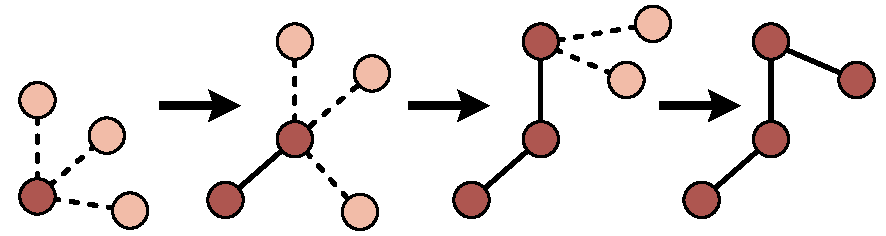
\includegraphics[width=0.9\textwidth]{figures/images/cbmc}
    \caption{Illustration of a single configurational bias Monte Carlo move. A
    linear molecule is regrown step by step. At each step, the position for the
    next atom is picked at random, depending on the position of all the
    previous atoms.}
    \label{fig:cbmc}
\end{figure}

The main issue with configuration bias Monte Carlo is that it requires
knowledge of all the separated intra-molecular interaction terms to be able to
generate the position of the next atom while maintaining detailed balance; and
not only the global energy change as for simpler moves. It is also harder to use
it for even the simplest branched molecules.

Flexible nanoporous materials add another level of difficulty for efficient
Monte Carlo simulations. Some of them display collective behavior linked to
global deformations of the simulation cell, such as breathing or gate-opening.
Here, the volume of the simulation cell changes as the linkers rotate and move,
thus needing Monte Carlo moves able to sample both the collective rotation of
linkers and the changes in the unit cell shape and volume. It is possible to use
molecular dynamics instead of Monte Carlo to explore the response of the
material to external stress, as molecular dynamics simulations are very
efficient when sampling collective behaviors. But when the stress is created by
adsorbed molecules in a variable number (for simulations with fixed chemical
potential), we need to use grand canonical Monte Carlo (molecular dynamics is
not suited for simulations in the grand canonical ensemble, see
section~\ref{sec:gcmd}). Hybrid Monte Carlo is a technique that can bridge the
gap between traditional Monte Carlo and molecular dynamics, bringing the ability
to sample such collective motions to a Monte Carlo simulation\cite{Rogge2019}.

In addition to being able to improve the sampling efficiency of Monte Carlo
simulations, Hybrid Monte Carlo can bring the power of non-physical moves in
simulations usually relying on molecular dynamics. For example, the study of
large bio-molecules --- the typical example is the simulation of protein folding
--- is often limited by the time scale at which the simulation can produce new
conformations, decorrelated from the previous ones\cite{Izaguirre2004}. Monte
Carlo can help reduce this time by allowing jumps from one conformation to
another, and incorporate domain-specific knowledge (which part of the protein
can rotate, which parts will move together) to improve simulation efficiency.

Another area that can see improvements by incorporating non-physical moves is
the simulation of diluted aqueous environments, such as the salt and pH
environment around proteins. The pH of human blood is constant around 7.4,
meaning that both \ce{HO-} and \ce{H+} ions are only present at a concentration
around \SI{e-7}{mol/L}. If we want to simulate a realistic pH environment, we
need to simulate more than 500 million water molecule for each \ce{HO-} or
\ce{H+} ion. In addition to that, because the surface of proteins can carry
non-neutral charges, the local ion concentration can depart from the measured,
global concentration in blood plasma or cell's cytoplasm. Grand Canonical and
semi-Grand Canonical Monte Carlo moves used together with Hybrid Monte Carlo can
bring realistic salt and pH condition to these simulations\cite{Ross2018}.

\subsection{Mixing molecular dynamics and Monte Carlo}

Hybrid Monte Carlo was first devised in 1987 by \citeauthor{Duane1987} for
calculations in lattice quantum chromodynamics \cite{Duane1987}. It was then
adapted to condensed matter molecular simulation by \citeauthor{Mehlig1992} in
1992\cite{Mehlig1992}. The central idea is to use a short molecular dynamics
simulation (around 10 steps) to generate a new conformation for the Markov
chain. Once the molecular dynamics simulation finished, the final step is
considered as a trial conformation, and accepted or rejected with the adapted
Metropolis criterion.

One global move in \emph{configuration space} consists in propagating the system
through \emph{phase space} for a fixed number of steps using some integration
scheme $\psi_{\delta t}$ of Hamilton's equations. $\psi_{\delta t}$ depends on
the integration time step $\delta t$ and the Hamiltonian of the system
$\mathcal{H}$; and maps the initial configuration $(\r, \v)$ in phase space to
the final one $(\r', \v')$:
\[\begin{array}{llcl}
    \psi_{\delta t} : & \mathbb{R}^{6N} & \longrightarrow & \mathbb{R}^{6N} \\
                      & (\r, \v)        & \longmapsto     & \psi_{\delta t}(\r, \v) \equiv (\r', \v')
\end{array}\]

Since the usual Monte Carlo scheme does not use (or propagate) the atomic
velocities, we need to generate new velocities before starting the molecular
dynamics simulation. We choose to generate them randomly according to the the
canonical ensemble distribution at temperature $T$:
\[ \mathcal{P}_T(\v) \propto \exp\left(- \beta \sum_i \frac 12 m_i \v_i^2 \right)\]

Following the same notations as in chapter~\ref{sec:molsim}, because the time
integration is deterministic, the probability $\alpha(\r \to \r')$ to generate a
given conformation $\r'$ starting from $\r$ is the same as the probability to
generate a specific set of initial velocities $\mathcal{P}_T(\v)$:
\[ \alpha(\r \to \r')\ \d\r' = \mathcal{P}_T(\v) \ \d\v \]

The error in energy conservation made by the propagator $\psi_{\delta t}$ is
called the discretization error $\delta \mathcal{H}$. This value is associated
with the numeric integration scheme used by the molecular simulation, and depends
only on $\delta t$ and the number of steps used to propagate the system with
molecular dynamics.
\[\delta \mathcal{H} = \mathcal{H}(\r', \v') - \mathcal{H}(\r, \v)\]
If we use an acceptation probability that depends on the discretization error
$\delta \mathcal{H}$:
\[\text{acc}\left[(\r, \v) \to (\r', \v')\right] = \min\left(1, e^{-\beta \delta \mathcal{H}}\right), \]
we can show that the resulting Monte Carlo move respects the detailed balance,
provided that the integration scheme $\psi_{\delta t}$ is both \emph{time
reversible} and \emph{symplectic}.
\[\begin{array}{lcllll}
    \mathcal{P}(\r)\ \pi(\r \to \r') \ \d\r\d\v   &=& \mathcal{P}(\r)  & \mathcal{P}_T(\v)  & \text{acc}\kern-0.5ex\left((\r, \v) \to \psi_{\delta t}(\r, \v)\right)      & \d\r\d\v \\
    \text{\footnotesize \itshape see below}       &=& \mathcal{P}(\r') & \mathcal{P}_T(\v') & \text{acc}\kern-0.5ex\left(\psi_{\delta t}(\r, \v) \to (\r, \v)\right)      & \d\r\d\v \\
    \text{\footnotesize \itshape time reversible} &=& \mathcal{P}(\r') & \mathcal{P}_T(\v') & \text{acc}\kern-0.5ex\left((\r', \v') \to \psi_{-\delta t}(\r', \v')\right) & \d\r\d\v \\
    \text{\footnotesize \itshape symplectic}      &=& \mathcal{P}(\r') & \mathcal{P}_T(\v') & \text{acc}\kern-0.5ex\left((\r', \v') \to \psi_{-\delta t}(\r', \v')\right) & \d\r'\d\v' \\
                                                  &=& \mathcal{P}(\r') & \multicolumn{2}{l}{\pi(\r' \to \r) \ \d\r'\d\v'}
\label{eq:hmc-demonstration}
\end{array}\]
The first step in the above demonstration comes from the mathematical identity
\[e^{-\beta\mathcal{H}(\r, \v)} \min\kern-0.5ex\left(1, e^{-\beta \delta \mathcal{H}}\right) = e^{-\beta\mathcal{H}(\r', \v')} \min\kern-0.5ex\left(e^{\, \beta \delta \mathcal{H}}, 1\right). \]

It is worth noting that even though the molecular dynamics simulation evolves in
the microcanonical $NVE$ ensemble, the overall HMC simulation is sampling the
canonical $NVT$ ensemble. This allows using HMC simulations as a rigorous way to
sample the $NVT$ ensemble using molecular dynamics.

\subsubsection{Constant pressure simulations}

There are two ways to use Hybrid Monte Carlo simulations to sample the
isobaric-isothermal $NPT$ ensemble. The first one is to use separate moves to
change the volume and the particles' positions --- the former using standard
Monte Carlo moves and the latter relying on hybrid moves. This is the usual way
of running $NPT$ simulations with Monte Carlo, with some added hybrid moves to
sample the configuration space at different fixed volumes. While doing so is
simpler from an implementation point of view, it can be less efficient when the
changes in volume are coupled to local deformations of the system, which is
often the case in flexible nanoporous materials.

Another possibility is to use the hybrid moves to sample both the volume changes
and the particles' displacements. The same construction described above can be
used to create an hybrid move that sample the $NPT$ ensemble. The molecular
dynamics integrator now maps the initial position in phase space including the
volume $V$ $(V, \r, \v)$ to a new position in phase space $(V', \r', \v')$. If
the integrator is deterministic, the probability to generate a specific new
state from the initial one, $\alpha\left[(V, \r) \to (V', \r')\right]$, is still
the same as the probability to generate the initial velocities
$\mathcal{P}_T(\v)$. Provided the integrator is time reversible and symplectic,
the same demonstration as in equation~\eqref{eq:hmc-demonstration} applies by
adapting the acceptance criterion to
\[\text{acc}\left[(V, \r, \v) \to (V', \r', \v')\right] = \min\left(1, e^{-\beta \delta \mathcal{H} - \beta\ P \Delta V}\right)\]

If an extended Lagrangian integrator such as the one proposed by Andersen (see
reference~\cite{Andersen1980}) is used, the momentum of the fictitious external
piston should also be included in both the probability of creating a new state
$\alpha((V, \r) \to (V', \r'))$ and in the Hamiltonian part of the acceptance
criterion\cite{Faller2002, FernandezPendas2014}.

Again, we should note that the molecular dynamics simulation only samples the
is\-enthalpic-iso\-baric $NPH$ ensemble, and the Monte Carlo acceptance
criterion ensures sampling of the isobaric-isothermal $NPT$ ensemble. Actually,
the molecular dynamics does not even need to sample an accurate $NPH$ ensemble,
only to generate new states with different volume and following the above
properties of being deterministic, time-reversible and symplectic. The
Metropolis acceptance criterion ensures that the correct ensemble will be
sampled. However, care must still be taken to minimize the enthalpy drift
$\delta \mathcal{H} + P \Delta V$ during the simulation to maintain a high
acceptance rate for hybrid moves.

\subsubsection{Osmotic simulations}

Once we are able to use hybrid Monte Carlo simulations to sample the $NPT$
ensemble, moving to the osmotic $N_\text{host}\,\mu\,PT$ ensemble is
accomplished by adding insertion/deletion moves to allow the number of adsorbed
particles to vary. Earlier this year, \citeauthor{Rogge2019}\cite{Rogge2019} used
such hybrid Monte Carlo simulations to study the adsorption of noble gases, \ce{CO2}
and \ce{CH4} in MIL-53(Al) using the osmotic ensemble. They were able to reach
very good agreement with experimental measurements of adsorption isotherms and
predict the bi-stability and breathing of MIL-53(Al) upon adsorption.

Because the correctness of the sampled ensemble is validated by the Metropolis
criterion and the detailed balance, the short molecular dynamics simulations
used in hybrid moves are not required to produce the statistically correct
ensemble. This means that it should be possible to use an adapted Grand
Canonical Molecular Dynamics scheme to generate new trial conformation to be
accepted with the Metropolis criterion. To my knowledge, this as not been
attempted yet, but could improve insertion rate for osmotic simulations in dense
phases --- such as the simulation of intrusion in porous solids. Traditional
insertion/deletion moves suffer from a very low acceptance rate in dense phases
such as liquids, because molecules are already densely packed and there is not
enough space to add new molecules. Grand canonical molecular dynamics can help
by progressively scaling the \emph{presence} of the new molecule up, allowing
its surroundings to relax.

Even if we have a simulation method able to sample the osmotic ensemble, we will
still need force fields able to accurately describe both the flexibility of the
materials and the interactions between the material and the fluids inside.
Developing such force field will require additional efforts, especially
considering the variability of structures of hybrid metal--organic materials,
and the inherent complexity of describing coordination bonds. Force field
parametrization methods based on machine learning --- such as the one I
presented in section~\ref{sec:classical-ff-parametrize} --- could be very
valuable for this endeavor.

\subsubsection{Related algorithms and methods}

In the last decade, some improvements to the simple hybrid Monte Carlo method
presented above have been proposed. Shadow Hybrid Monte
Carlo\cite{Izaguirre2004} relies on the existence and computability of a
\emph{shadow} Hamiltonian being propagated exactly (without any propagation
error) by $\psi_{\delta t}$ to improve the acceptance rate of hybrid moves, and
reconstruct \emph{a posteriori} the probabilities of each generated
conformation. Generalized Hybrid Monte Carlo\cite{Horowitz1991, Akhmatskaya2009,
Akhmatskaya2011} uses configurations in the phase space instead of conformations
in the Markov chain, keeping the velocities from one Monte Carlo move to
another. The different steps are still accepted or rejected by a Metropolis
criterion, and velocities are partially updated with new random values at each
step. The combination of these two approaches is called Generalized Shadow
Hybrid Monte Carlo, and implemented in the GROMACS simulation
software\cite{FernandezPendas2014}. Finally, tentatives to lift the symplectic
requirement on the integrator are at the origin of Compressible Generalized
Hybrid Monte Carlo\cite{Lan2015, Fang2014}. The core idea is to include the
Jacobian $\mathcal{J}_{\psi_{\delta t}}$ of the propagator in the probability
ratio of the acceptance test:
\[\text{acc}\left[(\r, \v) \to (\r', \v')\right] = \min\left(1, \frac{\mathcal{P}(\r', \v')}{\mathcal{P}(\r, \v)} \left|\mathcal{J}_{\psi_{\delta t}}\right|\right)\]
where $\mathcal{J}_{\psi_{\delta t}} = \text{det}\left[\partial \psi_{\delta t}
\,/\, \partial (\r, \v)\right]$. For a symplectic integrator,
$|\mathcal{J}_{\psi_{\delta t}}| = 1$, and we get back the standard hybrid Monte
Carlo scheme.

\subsection{Hybrid simulations in osmotic ensemble}

I used my implementation of hybrid Monte Carlo in Domino in a preliminary study
of the adsorption of methane \ce{CH4} in MOF-5 at \SI{300}{K}. I used a
simplified model of both MOF-5 and \ce{CH4} as Domino did not support computing
electrostatic interactions when I first implemented these algorithms. \ce{CH4}
molecules were approximated by Lennard-Jones spheres, using $\sigma =
\SI{3.737}{\AA}$ and $\epsilon = \SI{1.247}{kJ/mol}$. I used the Lennard-Jones
and intra-molecular terms from QuickFF\cite{Vanduyfhuys2015} to describe the
MOF, ignoring the atomic charges. While the resulting model is not an accurate
representation of MOF-5, it is still an interesting test case for the use of
hybrid Monte Carlo simulations in adsorption.

To obtain a full isotherm, I ran 8 simulations at different \ce{CH4} pressures.
Each simulation used two Monte Carlo moves: insertion/deletion of \ce{CH4}
taking the current pressure as the gas fugacity; and hybrid moves. The hybrid
moves used a Velocity-Verlet integrator with a timestep of \SI{1}{fs}, and a
Berendsen barostat setting the external pressure at the same value as the
\ce{CH4} fugacity and a time step of \SI{5}{ps}. I should point out that I used
the Berendsen barostat even if it is not symplectic nor time reversible, as it
was the only barostat implemented in Domino. Despite of its flaws, this barostat
is very common in the literature as it is the simplest possible choice. Again,
while the resulting simulation might not sample the adequate ensemble, it is
still an interesting check. Each simulation was propagated for a million of
Monte Carlo moves, using the first 250 000 moves as the equilibration period.
The resulting isotherm is shown in figure~\ref{fig:hmc-mof5} together with the
changes in unit cell volume as the pressure increases.

\begin{figure}[ht]
    \centering
    % GNUPLOT: LaTeX picture with Postscript
\begingroup
  \makeatletter
  \providecommand\color[2][]{%
    \GenericError{(gnuplot) \space\space\space\@spaces}{%
      Package color not loaded in conjunction with
      terminal option `colourtext'%
    }{See the gnuplot documentation for explanation.%
    }{Either use 'blacktext' in gnuplot or load the package
      color.sty in LaTeX.}%
    \renewcommand\color[2][]{}%
  }%
  \providecommand\includegraphics[2][]{%
    \GenericError{(gnuplot) \space\space\space\@spaces}{%
      Package graphicx or graphics not loaded%
    }{See the gnuplot documentation for explanation.%
    }{The gnuplot epslatex terminal needs graphicx.sty or graphics.sty.}%
    \renewcommand\includegraphics[2][]{}%
  }%
  \providecommand\rotatebox[2]{#2}%
  \@ifundefined{ifGPcolor}{%
    \newif\ifGPcolor
    \GPcolortrue
  }{}%
  \@ifundefined{ifGPblacktext}{%
    \newif\ifGPblacktext
    \GPblacktextfalse
  }{}%
  % define a \g@addto@macro without @ in the name:
  \let\gplgaddtomacro\g@addto@macro
  % define empty templates for all commands taking text:
  \gdef\gplbacktext{}%
  \gdef\gplfronttext{}%
  \makeatother
  \ifGPblacktext
    % no textcolor at all
    \def\colorrgb#1{}%
    \def\colorgray#1{}%
  \else
    % gray or color?
    \ifGPcolor
      \def\colorrgb#1{\color[rgb]{#1}}%
      \def\colorgray#1{\color[gray]{#1}}%
      \expandafter\def\csname LTw\endcsname{\color{white}}%
      \expandafter\def\csname LTb\endcsname{\color{black}}%
      \expandafter\def\csname LTa\endcsname{\color{black}}%
      \expandafter\def\csname LT0\endcsname{\color[rgb]{1,0,0}}%
      \expandafter\def\csname LT1\endcsname{\color[rgb]{0,1,0}}%
      \expandafter\def\csname LT2\endcsname{\color[rgb]{0,0,1}}%
      \expandafter\def\csname LT3\endcsname{\color[rgb]{1,0,1}}%
      \expandafter\def\csname LT4\endcsname{\color[rgb]{0,1,1}}%
      \expandafter\def\csname LT5\endcsname{\color[rgb]{1,1,0}}%
      \expandafter\def\csname LT6\endcsname{\color[rgb]{0,0,0}}%
      \expandafter\def\csname LT7\endcsname{\color[rgb]{1,0.3,0}}%
      \expandafter\def\csname LT8\endcsname{\color[rgb]{0.5,0.5,0.5}}%
    \else
      % gray
      \def\colorrgb#1{\color{black}}%
      \def\colorgray#1{\color[gray]{#1}}%
      \expandafter\def\csname LTw\endcsname{\color{white}}%
      \expandafter\def\csname LTb\endcsname{\color{black}}%
      \expandafter\def\csname LTa\endcsname{\color{black}}%
      \expandafter\def\csname LT0\endcsname{\color{black}}%
      \expandafter\def\csname LT1\endcsname{\color{black}}%
      \expandafter\def\csname LT2\endcsname{\color{black}}%
      \expandafter\def\csname LT3\endcsname{\color{black}}%
      \expandafter\def\csname LT4\endcsname{\color{black}}%
      \expandafter\def\csname LT5\endcsname{\color{black}}%
      \expandafter\def\csname LT6\endcsname{\color{black}}%
      \expandafter\def\csname LT7\endcsname{\color{black}}%
      \expandafter\def\csname LT8\endcsname{\color{black}}%
    \fi
  \fi
    \setlength{\unitlength}{0.0500bp}%
    \ifx\gptboxheight\undefined%
      \newlength{\gptboxheight}%
      \newlength{\gptboxwidth}%
      \newsavebox{\gptboxtext}%
    \fi%
    \setlength{\fboxrule}{0.5pt}%
    \setlength{\fboxsep}{1pt}%
\begin{picture}(7360.00,2820.00)%
    \gplgaddtomacro\gplbacktext{%
      \csname LTb\endcsname%%
      \put(543,595){\makebox(0,0)[r]{\strut{}$0$}}%
      \csname LTb\endcsname%%
      \put(543,886){\makebox(0,0)[r]{\strut{}$5$}}%
      \csname LTb\endcsname%%
      \put(543,1177){\makebox(0,0)[r]{\strut{}$10$}}%
      \csname LTb\endcsname%%
      \put(543,1468){\makebox(0,0)[r]{\strut{}$15$}}%
      \csname LTb\endcsname%%
      \put(543,1760){\makebox(0,0)[r]{\strut{}$20$}}%
      \csname LTb\endcsname%%
      \put(543,2051){\makebox(0,0)[r]{\strut{}$25$}}%
      \csname LTb\endcsname%%
      \put(543,2342){\makebox(0,0)[r]{\strut{}$30$}}%
      \csname LTb\endcsname%%
      \put(543,2633){\makebox(0,0)[r]{\strut{}$35$}}%
      \csname LTb\endcsname%%
      \put(645,409){\makebox(0,0){\strut{}$0$}}%
      \csname LTb\endcsname%%
      \put(1100,409){\makebox(0,0){\strut{}$10$}}%
      \csname LTb\endcsname%%
      \put(1554,409){\makebox(0,0){\strut{}$20$}}%
      \csname LTb\endcsname%%
      \put(2009,409){\makebox(0,0){\strut{}$30$}}%
      \csname LTb\endcsname%%
      \put(2464,409){\makebox(0,0){\strut{}$40$}}%
      \csname LTb\endcsname%%
      \put(2918,409){\makebox(0,0){\strut{}$50$}}%
      \csname LTb\endcsname%%
      \put(3373,409){\makebox(0,0){\strut{}$60$}}%
    }%
    \gplgaddtomacro\gplfronttext{%
      \csname LTb\endcsname%%
      \put(153,1614){\rotatebox{-270}{\makebox(0,0){\strut{}intake (\% wt)}}}%
      \csname LTb\endcsname%%
      \put(2009,130){\makebox(0,0){\strut{}pressure (bar)}}%
    }%
    \gplgaddtomacro\gplbacktext{%
      \csname LTb\endcsname%%
      \put(4427,595){\makebox(0,0)[r]{\strut{}$16.8$}}%
      \csname LTb\endcsname%%
      \put(4427,1003){\makebox(0,0)[r]{\strut{}$17$}}%
      \csname LTb\endcsname%%
      \put(4427,1410){\makebox(0,0)[r]{\strut{}$17.2$}}%
      \csname LTb\endcsname%%
      \put(4427,1818){\makebox(0,0)[r]{\strut{}$17.4$}}%
      \csname LTb\endcsname%%
      \put(4427,2225){\makebox(0,0)[r]{\strut{}$17.6$}}%
      \csname LTb\endcsname%%
      \put(4427,2633){\makebox(0,0)[r]{\strut{}$17.8$}}%
      \csname LTb\endcsname%%
      \put(4529,409){\makebox(0,0){\strut{}$0$}}%
      \csname LTb\endcsname%%
      \put(4950,409){\makebox(0,0){\strut{}$10$}}%
      \csname LTb\endcsname%%
      \put(5370,409){\makebox(0,0){\strut{}$20$}}%
      \csname LTb\endcsname%%
      \put(5791,409){\makebox(0,0){\strut{}$30$}}%
      \csname LTb\endcsname%%
      \put(6212,409){\makebox(0,0){\strut{}$40$}}%
      \csname LTb\endcsname%%
      \put(6632,409){\makebox(0,0){\strut{}$50$}}%
      \csname LTb\endcsname%%
      \put(7053,409){\makebox(0,0){\strut{}$60$}}%
    }%
    \gplgaddtomacro\gplfronttext{%
      \csname LTb\endcsname%%
      \put(3833,1614){\rotatebox{-270}{\makebox(0,0){\strut{}volume (\si{nm^3})}}}%
      \csname LTb\endcsname%%
      \put(5791,130){\makebox(0,0){\strut{}pressure (bar)}}%
    }%
    \gplbacktext
    \put(0,0){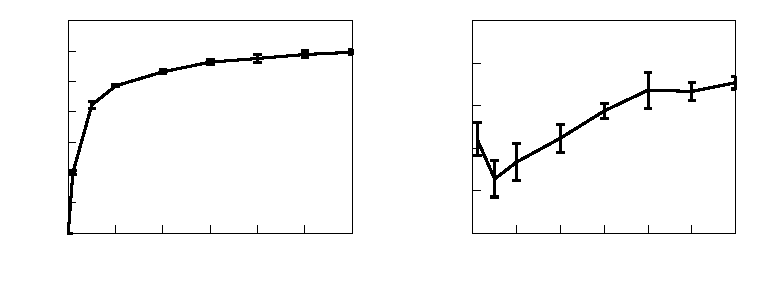
\includegraphics{hmc-mof5}}%
    \gplfronttext
  \end{picture}%
\endgroup

    \caption{Hybrid Grand Canonical Monte Carlo simulations results for the
    adsorption of methane in a simplified MOF-5 model. (left) adsorption
    isotherm at \SI{300}{K}, (right) volume change during adsorption.}
    \label{fig:hmc-mof5}
\end{figure}

The resulting isotherm is a simple type I isotherm, as expected for the
adsorption of methane in MOF-5. Contrary to standard GCMC simulations, this
isotherm incorporates flexibility effects. More interesting is the non-monotonous
behavior of the curve of volume deformations as a function of pressure. We first
see a small contraction of the unit cell at low loading, before the expected
increase at higher pressures. This contract--expand behavior is reminiscent of
sorption-induced deformation in other porous materials\cite{Balzer2013,
Mouhat2015}: the presence of few molecules inside the pores induces a
\emph{softening} and a contraction of the whole system. Another way to look at
this phenomenon is to envision the molecules inside the pore \emph{pulling} on
the pores' wall.

It is remarkable to see that such a simplistic model of the MOF is able to
reproduce this relatively complex behavior. In order to improve the model and
predictive possibilities of hybrid Monte Carlo simulations, I needed to
implement a way to compute electrostatic interactions. In the next section, I
will discuss two methods one can use to compute these interactions in the
presence of periodic boundary conditions.

\newpage
\section{Computation of electrostatic energy in classical simulations}
\label{sec:electrostatic}

Classical force fields represent the energy of an atomic system as a sum of
multiple contributions, including dispersion and short-range repulsion,
intra-molecular interactions and electrostatic interactions. In the last case,
atoms are often identified to point charges, interacting through a Coulombic
potential. For two atoms $i$ and $j$ carrying charges $q_i$ and $q_j$, at a
distance $r$ from one another, this potential reads:
\[ V(r) = \frac{q_i q_j}{4 \pi \epsilon_0 r}.\]
In the remaining of this chapter, I will be using units such that $4 \pi
\epsilon_0 = 1$.

\subsection{The problem}

As presented in section~\ref{sec:pbc}, we are limited in the size of systems we
can simulate with classical simulation methods. To remove the size and surface
effects arising from the relatively small number of simulated particles, most if
not all classical simulations use periodic boundary conditions. This means that
we are, in effect, simulating an infinite system, extending in all three
dimensions of space. All the inter-molecular interaction potentials decay to
zero as the distance between atoms goes to infinity. It is thus customary to use
a cutoff radius $r_c$ when computing the energy of a system: any interaction
between atoms further apart than this radius is supposed negligible, and set to
zero. This allows to speed up the calculation of energies in the simulations by
ignoring contributions between atoms that are too far apart. The error
$\epsilon$ arising from the use of a cutoff radius can be quantified --- using
$V(r)$ for the pair potential and $g(r)$ for the radial distribution function:
\[\epsilon = \int_{r_c}^\infty r^2 \ V(r) \ g(r)\ \d r. \]
Assuming isotropic density, and for a cutoff radius big enough so that $g(r)
\simeq 1$, we can compute this value --- also called \emph{long-range} or
\emph{tail} correction --- and use it to correct after the fact the energy and
pressure computed from a simulation.

Unfortunately, the above integral only converges if $V(r)$ goes to zero faster
than $1/r^3$, which is not the case for the electrostatic potential. In the
following, I will be describing two methods one can use to compute the
electrostatic interactions accurately in classical molecular simulations: Ewald
summation and Wolf summation. I implemented both in the Domino project, and I
will give some software implementation techniques I used to speed up energy and
forces computations.

\subsection{Ewald summation}

Ewald summation was proposed by Paul Peter Ewald in 1921\cite{Ewald1921}. The
core idea is to decompose the electrostatic potential using the identity:
\[ \frac{1}{r} = \frac{f(r)}{r} + \frac{1 - f(r)}{r}. \]
By choosing the right $f(r)$, one can create decompose $1/r$ potential into a
short-range, rapidly converging potential that can be computed with a cutoff
radius; and a long-range, smooth potential that will be computed in Fourier
space. While I am focusing here on electrostatic interaction, the Ewald
summation is a more general technique that can be used with other potentials.
The usual decomposition uses the error function $\erf$ and the complementary
error function $\erfc$:
\[\erf(x) = \frac{2}{\sqrt\pi} \int_0^x e^{-t^2} \d t \hskip3em \erfc(x) = 1 - \erf(x)\]
The three functions are represented in figure~\ref{fig:ewald:erf}, were we can
see that $\erfc(r)/r$ goes to zero faster than $1/r$, and that $\erf(r)/r$ is
very smooth, and can be prolonged to a finite value on $r = 0$.

\begin{figure}[ht]
    \centering
    % GNUPLOT: LaTeX picture with Postscript
\begingroup
  \makeatletter
  \providecommand\color[2][]{%
    \GenericError{(gnuplot) \space\space\space\@spaces}{%
      Package color not loaded in conjunction with
      terminal option `colourtext'%
    }{See the gnuplot documentation for explanation.%
    }{Either use 'blacktext' in gnuplot or load the package
      color.sty in LaTeX.}%
    \renewcommand\color[2][]{}%
  }%
  \providecommand\includegraphics[2][]{%
    \GenericError{(gnuplot) \space\space\space\@spaces}{%
      Package graphicx or graphics not loaded%
    }{See the gnuplot documentation for explanation.%
    }{The gnuplot epslatex terminal needs graphicx.sty or graphics.sty.}%
    \renewcommand\includegraphics[2][]{}%
  }%
  \providecommand\rotatebox[2]{#2}%
  \@ifundefined{ifGPcolor}{%
    \newif\ifGPcolor
    \GPcolortrue
  }{}%
  \@ifundefined{ifGPblacktext}{%
    \newif\ifGPblacktext
    \GPblacktextfalse
  }{}%
  % define a \g@addto@macro without @ in the name:
  \let\gplgaddtomacro\g@addto@macro
  % define empty templates for all commands taking text:
  \gdef\gplbacktext{}%
  \gdef\gplfronttext{}%
  \makeatother
  \ifGPblacktext
    % no textcolor at all
    \def\colorrgb#1{}%
    \def\colorgray#1{}%
  \else
    % gray or color?
    \ifGPcolor
      \def\colorrgb#1{\color[rgb]{#1}}%
      \def\colorgray#1{\color[gray]{#1}}%
      \expandafter\def\csname LTw\endcsname{\color{white}}%
      \expandafter\def\csname LTb\endcsname{\color{black}}%
      \expandafter\def\csname LTa\endcsname{\color{black}}%
      \expandafter\def\csname LT0\endcsname{\color[rgb]{1,0,0}}%
      \expandafter\def\csname LT1\endcsname{\color[rgb]{0,1,0}}%
      \expandafter\def\csname LT2\endcsname{\color[rgb]{0,0,1}}%
      \expandafter\def\csname LT3\endcsname{\color[rgb]{1,0,1}}%
      \expandafter\def\csname LT4\endcsname{\color[rgb]{0,1,1}}%
      \expandafter\def\csname LT5\endcsname{\color[rgb]{1,1,0}}%
      \expandafter\def\csname LT6\endcsname{\color[rgb]{0,0,0}}%
      \expandafter\def\csname LT7\endcsname{\color[rgb]{1,0.3,0}}%
      \expandafter\def\csname LT8\endcsname{\color[rgb]{0.5,0.5,0.5}}%
    \else
      % gray
      \def\colorrgb#1{\color{black}}%
      \def\colorgray#1{\color[gray]{#1}}%
      \expandafter\def\csname LTw\endcsname{\color{white}}%
      \expandafter\def\csname LTb\endcsname{\color{black}}%
      \expandafter\def\csname LTa\endcsname{\color{black}}%
      \expandafter\def\csname LT0\endcsname{\color{black}}%
      \expandafter\def\csname LT1\endcsname{\color{black}}%
      \expandafter\def\csname LT2\endcsname{\color{black}}%
      \expandafter\def\csname LT3\endcsname{\color{black}}%
      \expandafter\def\csname LT4\endcsname{\color{black}}%
      \expandafter\def\csname LT5\endcsname{\color{black}}%
      \expandafter\def\csname LT6\endcsname{\color{black}}%
      \expandafter\def\csname LT7\endcsname{\color{black}}%
      \expandafter\def\csname LT8\endcsname{\color{black}}%
    \fi
  \fi
    \setlength{\unitlength}{0.0500bp}%
    \ifx\gptboxheight\undefined%
      \newlength{\gptboxheight}%
      \newlength{\gptboxwidth}%
      \newsavebox{\gptboxtext}%
    \fi%
    \setlength{\fboxrule}{0.5pt}%
    \setlength{\fboxsep}{1pt}%
\begin{picture}(4520.00,2820.00)%
    \gplgaddtomacro\gplbacktext{%
      \csname LTb\endcsname%%
      \put(915,49){\makebox(0,0)[l]{\strut{}$1 / \alpha$}}%
    }%
    \gplgaddtomacro\gplfronttext{%
      \csname LTb\endcsname%%
      \put(3243,2353){\makebox(0,0)[r]{\strut{}$1 / r$}}%
      \csname LTb\endcsname%%
      \put(3243,2028){\makebox(0,0)[r]{\strut{}$\erfc(\alpha r) / r$}}%
      \csname LTb\endcsname%%
      \put(3243,1703){\makebox(0,0)[r]{\strut{}$\erf(\alpha r) / r$}}%
    }%
    \gplbacktext
    \put(0,0){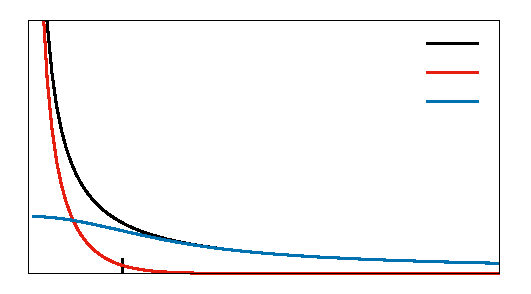
\includegraphics{ewald-erf}}%
    \gplfronttext
  \end{picture}%
\endgroup

    \caption{Shape of the functions involved in Ewald summation: $1/r$, $\erfc(\alpha r) / r$,
    and $\erf(\alpha r) / r$.}
    \label{fig:ewald:erf}
\end{figure}

In practice, a damping parameter $\alpha$ is used to tune the distance at which
$\erfc\,(\alpha r) / r$ becomes dominant over $\erf\,(\alpha r) / r$. The
potential to be computed is given by:
\[ V(r) = q_i q_j \left[\frac{\erfc(\alpha r)}{r} + \frac{\erf(\alpha r)}{r} \right].\]
The total energy of the system is a sum over all possible pairs, and can be
decomposed as a short-range contribution $U_\text{short}$ (containing the
$\erfc$ terms) and a long-range contribution $U_\text{long}$ (containing the
$\erf$ terms):
\[ U = \frac12 \sum_{i\neq j}^\infty q_i q_j \frac{\erfc(\alpha r_{ij})}{r_{ij}} + \frac12 \sum_{i\neq j}^\infty q_i q_j \frac{\erf(\alpha r_{ij})}{r_{ij}};\]
\[ U = U_\text{short} + U_\text{long}\]
The short-range contribution sum can be evaluated directly (in \emph{real
space}) using a cutoff radius $r_c$, as it decays faster than $1/r^3$:
\[ U_\text{short} = \frac12 \sum_{\substack{i\neq j \\ r_{ij} < r_c}} q_i q_j \frac{\erfc(\alpha r_{ij})}{r_{ij}}.\]

Concerning the long-range contribution, we can use the periodicity introduced by
periodic boundary conditions to our advantage: as the potential $\erf(\alpha
r)/r$ is relatively smooth, its Fourier transform will only contain a small
number of harmonics. This means it will converge rapidly in \emph{Fourier
space}.

First we make the sum fully periodic by adding the term for $i = j$, and
extending $\erf(\alpha r)/r$ in zero to $\alpha / \sqrt\pi$:
\[ U_\text{long} = \frac12 \sum_{i, j}^\infty q_i q_j \frac{\erf(\alpha r_{ij})}{r_{ij}} - \sum_i^N \frac{\alpha}{\sqrt\pi} q_i^2.\]
By taking the Fourier transform of the sum over all reciprocal lattice
translations $\vec k$, and after a bit of algebra, we get a simpler expression:
\[ U_\text{long} = \frac{\pi}{V} \int_0^\alpha \frac{1}{u^3} \d u \ \sum_{i,j} q_i q_j \ +\ \frac{2\pi}{V} \sum_{\vec k \neq 0}^\infty \frac{e^{-k^2 / 4 \alpha^2}}{k^2} \left|\sum_i^N q_i \ e^{\ j \vec k \cdot \r_i}\right|^2  \kern1ex  -\ \sum_i^N \frac{\alpha}{\sqrt\pi} q_i^2, \label{eq:ewald:long}\]
where $j$ is the imaginary number ($j^2 = -1$). The first integral in
equation~\eqref{eq:ewald:long} comes from the $\vec k = 0$ case, and is
infinite. This means that the energy is infinite unless $\sum_{i,j} q_i q_j$ is
null, \ie unless the simulated system is neutral. This makes sense, as an
infinite periodic charged system would have an infinite total charge. If this is
the case, we need to add an uniform background charge to ensure the neutrality
of the system.

The sum over $\vec k$ converges quickly, and is usually computed over a small
number of $\vec k$ vectors, using a cutoff in Fourier space $k_c$:
\[ U_\text{long} = \frac{2\pi}{V} \sum_{\substack{\vec k \neq 0\\[0.4ex] \vec k^2 < k_c^2}} \frac{e^{-k^2 / 4 \alpha^2}}{k^2} \left|\rho(\vec k)\right|^2  \kern1ex  -\ \sum_i^N \frac{\alpha}{\sqrt\pi} q_i^2.\]
\[\rho(\vec k) = \sum_i^N q_i \ e^{\ j \vec k \cdot \r_i}\]
The total energy in the Ewald formulation can include additional terms not
derived here, such as a correction for charged systems, and a correction for
intra-molecular interactions:
\[\begin{array}{lrc>{\displaystyle}l}
    \text{short-range interaction} & U &=& \frac12 \kern1em\sideset{}{^\ddagger}\sum_{i\neq j, \ r_{ij} < r_c} q_i q_j \frac{\erfc(\alpha r_{ij})}{r_{ij}} \\
    \text{long-range interaction} &&+& \frac{2\pi}{V} \sum_{\vec k \neq 0, \ \vec k^2 < k_c^2} \frac{e^{-k^2 / 4 \alpha^2}}{k^2} \left|\rho(\vec k)\right|^2 \\
    \text{self interaction} &&-& \sum_i^N \frac{\alpha}{\sqrt\pi} q_i^2 \\
    \text{molecular correction} &&-& \frac12 \sideset{}{^{\ddagger-1}}\sum_{i\neq j} q_i q_j \frac{\erf(\alpha r_{ij})}{r_{ij}} \\
    \text{charge correction} &&-& \frac{\pi}{2 \alpha^2 V} \left| \sum_i q_i \right|^2
    \label{eq:ewald}
\end{array} \]

The molecular correction comes from another trick used when fitting the
parameters of classical force fields. Electrostatic interactions between bonded
atoms are ignored, allowing the use of less stiff bonded potential. They are
typically completely ignored for 1-2 and 1-3 atoms, \ie atoms directly bonded
and atoms both bonded to a common central atom. 1-4 interaction can be included,
scaled down or ignored depending on the force field. In the above expression,
the $\sum^\ddagger$ symbol on the short-range term indicate that intra-molecular
contributions should be skipped or scaled down as necessary, and
$\sum^{\ddagger-1}$ indicate that the sum run over interactions that should be
excluded. For the long-range term, we only want to remove interaction between
atoms in the same molecule and in the same simulation box image. Instead of
changing the sum over the $\vec k$ vectors, we explicitly remove the
corresponding contribution --- leading to the molecular correction term in
equation~\eqref{eq:ewald}.

Following the same procedure, one can compute the force $\vec f_i$ acting on a
given atom at position $\r_i$, and the stress tensor contribution from
electrostatic interactions $\underline\sigma$.
\vskip-1.5\baselineskip
\[\renewcommand{\arraystretch}{3}\begin{array}{rc>{\displaystyle}l}
    \vec f_i &=& q_i \kern0.5em\sideset{}{^\ddagger}\sum_{j=1,\ r_{ij} < r_c}^N q_j \left[\frac{\erfc(\alpha r_{ij})}{r_{ij}} + \frac{2 \alpha}{\sqrt\pi} e^{-\alpha^2 r_{ij}^2} \right] \frac{\r_{ij}}{r_{ij}^2}\\
    &+& \frac{4\pi}{V} \sum_{\vec k \neq 0,\ \vec k^2 < k_c^2} \frac{e^{-k^2 / 4 \alpha^2}}{k^2} \mathcal{I}\kern-0.2ex m\left( e^{\,j \vec k \cdot \r_i} \rho(\vec k) \right) \vec k \\
    &+& \frac12 q_i \sideset{}{^{\ddagger-1}}\sum_j q_j \left[\frac{2\alpha}{\sqrt\pi} e^{-\alpha^2 r_{ij}^2} - \frac{\erf(\alpha r_{ij})}{r_{ij}} \right] \frac{\r_{ij}}{r_{ij}}
\end{array} \]
\vskip-\baselineskip
\[\renewcommand{\arraystretch}{3}\begin{array}{rc>{\displaystyle}l}
    3 V\ \underline\sigma &=& \frac12\kern0.5em\sideset{}{^\ddagger}\sum_{i\neq j,\ r_{ij} < r_c}^N q_i q_j \left[\frac{\erfc(\alpha r_{ij})}{r_{ij}} + \frac{2 \alpha}{\sqrt\pi} e^{-\alpha^2 r_{ij}^2} \right] \frac{\r_{ij}\otimes\r_{ij}}{r_{ij}^2}\\
    &+& \frac{4\pi}{V} \sum_{\vec k \neq 0,\ \vec k^2 < k_c^2} \frac{e^{-k^2 / 4 \alpha^2}}{k^2} \left|\rho(\vec k)\right|^2 \left[ \mathds{1} - \frac{2}{1/k^2 + 1/4\alpha^2} \vec k \otimes \vec k\right]  \\
    &+& \frac12 \sideset{}{^{\ddagger-1}}\sum_{i\neq j} q_i q_j \left[\frac{2\alpha}{\sqrt\pi} e^{-\alpha^2 r_{ij}^2} - \frac{\erf(\alpha r_{ij})}{r_{ij}} \right] \frac{\r_{ij}\otimes\r_{ij}}{r_{ij}} \\
\end{array} \]
Here, $\mathcal{I}\kern-0.2ex m$ is the imaginary part of a complex number. We
note that the self interaction and charge correction do not contribute to the
forces or stress.

\subsubsection{Implementation tricks}

When using the Ewald method for electrostatic potential computation, the
short-range contribution is the easiest to compute, as it behaves like a
standard pair potential. The long-range interaction is usually harder, and needs
more fine-tuning. A first easy improvement is to compute separately the factors
only depending on $\vec k$ vectors (such as $\exp(-k^2/4\alpha^2) / k^2$ and $2
/ (1 / k^2 + 1/4\alpha^2)$), and the Fourier transform of charge density
$\rho(\vec k)$. This allows re-using the factors as long as the unit cell does
not change, and only recompute the density. This also helps to improve
efficiency for Monte Carlo simulations, using the knowledge that only some atoms
moved to update $\rho(\vec k)$ (see figure~\ref{fig:mc-cache} and accompanying
text for more information on this strategy).

The choice of storage for the multiplicative factors and $\rho(\vec k)$ also has
a large impact on performance. As these quantities depend on $\vec k$ vectors,
it is natural to store them in three-dimensional arrays, corresponding to the
three components of the vector. But this strategy induces a lot of jumps when
accessing memory (called cache misses), lowering performance (see
section~\ref{sec:computer-model} for a performance model of modern computers).
A better strategy consists in using a first linear array to store the $\vec k$
vectors, each vector being associated with an index. Then, the multiplicative
factors and $\rho(\vec k)$ can also be stored in linear arrays, the
corresponding $\vec k$ vector for each entry being found by the entry index.
This drastically improves memory locality and performance of the calculation.

\subsection{Wolf summation}

The Wolf summation technique, proposed by the eponym author in
1999\cite{Wolf1999}, is based on the observation that the effective
electrostatic potential created by a multipole decays faster than $1/r$ at long
distances. For example, dipolar potential decays as $1/r^2$, quadrupolar moment
decays as $1/r^3$, and Wolf showed that complex multipoles such as crystals
create a potential that decays as $1/r^5$. It should thus be possible to use a
direct pair sum to evaluate it. The authors showed that the direct pair sum does
not converge when using spherical cutoff because the system included inside the
cutoff is not charge-neutral. They proposed to include a corrective term for the
remaining charge, effectively replacing the electrostatic potential by a shifted
potential:
\[V_{SP}(r_{ij}) = q_i q_j \left(\frac{1}{r_{ij}} - \frac{1}{r_c} \right)\]
The energy resulting from this potential is a good approximation of the true
electrostatic potential, while being a lot easier to compute. It gets closer to
the real energy as the cutoff distance is increased.

Because the naive shifted potential presented above requires relatively large
cutoff radius to offer a good approximation of the energy, the authors also
proposed to \emph{damp} the potential using the complementary error function.
This allow the use of smaller cutoff radius ($10 - \SI{20}{\AA}$), while still
being a good approximation of the true electrostatic potential. This
\emph{damped shifted potential} (DSP) --- and the corresponding force expression
--- are given by:
\[V_{DSP}(r_{ij}) = q_i q_j \left[\frac{\erfc(\alpha r_{ij})}{r_{ij}} - \frac{\erfc(\alpha r_c)}{r_c} \right]\]
\[\vec f_{DSP}(\vec r_{ij}) = q_i q_j \left[\frac{\erfc(\alpha r_{ij})}{r_{ij}^2} + \frac{2\alpha}{\sqrt{\pi}} \frac{\exp(-\alpha^2 r_{ij}^2)}{r_{ij}}\right] \frac{\vec r_{ij}}{r_{ij}},\]
where $\alpha$ is the damping parameter. This expression for the forces presents
a discontinuity at $r_{ij} = r_c$, which can introduce artifacts in molecular
dynamics simulation as particles enter or leave the cutoff sphere.

In 2006, \citeauthor{Fennell2006}\cite{Fennell2006} proposed to remove this
discontinuity by changing the potential to:
\[V_{DSF}(r_{ij}) = q_i q_j \left[\frac{\erfc(\alpha r_{ij})}{r_{ij}} - \frac{\erfc(\alpha r_c)}{r_c} + (r_{ij} - r_c) \frac{\partial V_{DSP}(r_{ij})}{\partial r_{ij}}(r_c)\right].\]
This approach gives us the \emph{damped shifted force} (DSF) formulation of Wolf
potential:
\[V_{DSF}(r_{ij}) = q_i q_j \left[\frac{\erfc(\alpha r_{ij})}{r_{ij}} - \frac{\erfc(\alpha r_c)}{r_c} + \left(\frac{\erfc(\alpha r_c)}{r_c^2} + \frac{2\alpha}{\sqrt{\pi}} \frac{\exp(-\alpha^2 r_c^2)}{r_c}\right) (r_{ij} - r_c)\right]\]
\[\vec f_{DSF}(\vec r_{ij}) = q_i q_j \left[\frac{\erfc(\alpha r_{ij})}{r_{ij}^2} + \frac{2\alpha}{\sqrt{\pi}} \frac{\exp(-\alpha^2 r_{ij}^2)}{r_{ij}} - \frac{\erfc(\alpha r_c)}{r_c^2} - \frac{2\alpha}{\sqrt{\pi}} \frac{\exp(-\alpha^2 r_c^2)}{r_c}\right] \frac{\vec r_{ij}}{r_{ij}}\]
\citeauthor{Fennell2006} also compared the these approaches on a large set
of systems, and concluded that the DSF approach is able to reproduce the forces
computed by Ewald summation very well with a damping parameter $\alpha =
\SI{0.2}{\AA^{-1}}$; while the DSP approach was able to reproduce energies using
the same damping parameter. They suggest using the DSP approach for Monte Carlo
simulation, and the DSF approach for molecular dynamics.

\subsection{Comparing Ewald and Wolf summations}

I implemented both the DSP and the DSF formulation of Wolf summation in
Domino. As they are based on sums of pair terms, they were much easier to
implement and integrate with Monte Carlo energy caching than Ewald summation.
Being simpler, the computation time for both energy and forces is smaller for
Wolf summation than for Ewald: for a small system containing 50 water molecules,
forces computation takes \SI{755}{\micro s} with Wolf, and \SI{1810}{\micro s}
with Ewald (respectively \SI{755}{\micro s} and \SI{860}{\micro s} for the
energy).

To check that my implementation of both Ewald and Wolf was correct, and to
compare their behavior in simple cases, I ran simulations in the $NVT$ ensemble
of NaCl in crystalline form at \SI{300}{K} and molten at \SI{2000}{K} using both
Domino and LAMMPS. I ran both Monte Carlo simulations, and molecular dynamics
simulations with Domino. I also ran molecular dynamics with LAMMPS as a
reference implementation. The molecular dynamics used a time step of \SI{1}{fs}
and a Berendsen thermostat to fix the temperature, with a thermostat time
constant of \SI{100}{fs}. Both Ewald and Wolf simulations used a cutoff radius
of \SI{11}{\AA} and a damping parameter $\alpha$ of \SI{0.29}{\AA^{-1}}. The
Ewald simulation considered $\vec k$ vectors up to 10 translations in reciprocal
space.

The system contained 256 \ce{Na+} and 256 \ce{Cl-} atoms, placed on a
face-centered cubic lattice, in a cubic simulation cell of \SI{22.56}{\AA}. The
molten NaCl simulations were started from the same conformation, placed into a
bigger unit cell of \SI{25.38}{\AA}. The atoms interacted through both
electrostatic and Lennard-Jones potentials, using parameters from
reference~\cite{Mao2012}. From these simulations, I extracted the average
pressure and potential energy, which are presented in
table~\ref{tab:ewald-vs-wolf}.

\begin{table}[ht]
    \def\mr#1#2{\multirow{#1}{*}{#2}}
    \caption{Energy and pressure ($\pm$ standard deviation) for multiple
    simulations comparing Ewald and Wolf on crystalline and molten NaCl. MC
    denotes Monte Carlo simulations, and MD molecular dynamics.}
    \label{tab:ewald-vs-wolf}
    \begin{tabular}{c c c c c c}
        \toprule
        Software & System  & Potential & Simulation & Energy (\si{kJ/mol}) & Pressure (bar) \\
        \midrule
        \mr{4}{LAMMPS} & \mr{2}{Crystal} &    Ewald  &    MD      & -203419 $\pm$ 45  & 13494 $\pm$ 302  \\
                       &                 &    Wolf   &    MD      & -203428 $\pm$ 45  & 13724 $\pm$ 297  \\
                       & \mr{2}{Molten}  &    Ewald  &    MD      & -182283 $\pm$ 345 & 15971 $\pm$ 1812 \\
                       &                 &    Wolf   &    MD      & -182424 $\pm$ 355 & 17977 $\pm$ 1770 \\
        \midrule
        \mr{8}{Domino} & \mr{4}{Crystal} &    Ewald  &    MD      & -203470 $\pm$ 53 & 13431 $\pm$ 229 \\
                       &                 &    Ewald  &    MC      & -203511 $\pm$ 62 & 13064 $\pm$ 383 \\
                       &                 &    Wolf   &    MD      & -86714 $\pm$ 69 & 13909 $\pm$ 355 \\
                       &                 &    Wolf   &    MC      & -86723 $\pm$ 69 & 13658 $\pm$ 455 \\
                       & \mr{4}{Molten}  &    Ewald  &    MD      & -182310 $\pm$ 278 & 15527 $\pm$ 1676 \\
                       &                 &    Ewald  &    MC      & -182818 $\pm$ 367 & 15090 $\pm$ 1620 \\
                       &                 &    Wolf   &    MD      & -65803 $\pm$ 306 & 18440 $\pm$ 1306 \\
                       &                 &    Wolf   &    MC      & -65785 $\pm$ 359 & 17686 $\pm$ 2054 \\
        \bottomrule
    \end{tabular}
\end{table}

First, we can see that my implementation of Ewald gives the same average values
for energy and pressure than LAMMPS, both for crystalline and molten NaCl; and
both for molecular dynamics and Monte Carlo simulations. My implementation of
Wolf also gives the same results with molecular dynamics and Monte Carlo, and
the same pressures as LAMMPS. Strangely, it does not give the same average
energies as LAMMPS, maybe because LAMMPS chooses a different energy origin.
This does not mean that my implementation is incorrect, as energies are only
defined up to an additive constant, but the origin of this difference should be
investigated further.

\begin{figure}[b]
    \centering
    % GNUPLOT: LaTeX picture with Postscript
\begingroup
  \makeatletter
  \providecommand\color[2][]{%
    \GenericError{(gnuplot) \space\space\space\@spaces}{%
      Package color not loaded in conjunction with
      terminal option `colourtext'%
    }{See the gnuplot documentation for explanation.%
    }{Either use 'blacktext' in gnuplot or load the package
      color.sty in LaTeX.}%
    \renewcommand\color[2][]{}%
  }%
  \providecommand\includegraphics[2][]{%
    \GenericError{(gnuplot) \space\space\space\@spaces}{%
      Package graphicx or graphics not loaded%
    }{See the gnuplot documentation for explanation.%
    }{The gnuplot epslatex terminal needs graphicx.sty or graphics.sty.}%
    \renewcommand\includegraphics[2][]{}%
  }%
  \providecommand\rotatebox[2]{#2}%
  \@ifundefined{ifGPcolor}{%
    \newif\ifGPcolor
    \GPcolortrue
  }{}%
  \@ifundefined{ifGPblacktext}{%
    \newif\ifGPblacktext
    \GPblacktextfalse
  }{}%
  % define a \g@addto@macro without @ in the name:
  \let\gplgaddtomacro\g@addto@macro
  % define empty templates for all commands taking text:
  \gdef\gplbacktext{}%
  \gdef\gplfronttext{}%
  \makeatother
  \ifGPblacktext
    % no textcolor at all
    \def\colorrgb#1{}%
    \def\colorgray#1{}%
  \else
    % gray or color?
    \ifGPcolor
      \def\colorrgb#1{\color[rgb]{#1}}%
      \def\colorgray#1{\color[gray]{#1}}%
      \expandafter\def\csname LTw\endcsname{\color{white}}%
      \expandafter\def\csname LTb\endcsname{\color{black}}%
      \expandafter\def\csname LTa\endcsname{\color{black}}%
      \expandafter\def\csname LT0\endcsname{\color[rgb]{1,0,0}}%
      \expandafter\def\csname LT1\endcsname{\color[rgb]{0,1,0}}%
      \expandafter\def\csname LT2\endcsname{\color[rgb]{0,0,1}}%
      \expandafter\def\csname LT3\endcsname{\color[rgb]{1,0,1}}%
      \expandafter\def\csname LT4\endcsname{\color[rgb]{0,1,1}}%
      \expandafter\def\csname LT5\endcsname{\color[rgb]{1,1,0}}%
      \expandafter\def\csname LT6\endcsname{\color[rgb]{0,0,0}}%
      \expandafter\def\csname LT7\endcsname{\color[rgb]{1,0.3,0}}%
      \expandafter\def\csname LT8\endcsname{\color[rgb]{0.5,0.5,0.5}}%
    \else
      % gray
      \def\colorrgb#1{\color{black}}%
      \def\colorgray#1{\color[gray]{#1}}%
      \expandafter\def\csname LTw\endcsname{\color{white}}%
      \expandafter\def\csname LTb\endcsname{\color{black}}%
      \expandafter\def\csname LTa\endcsname{\color{black}}%
      \expandafter\def\csname LT0\endcsname{\color{black}}%
      \expandafter\def\csname LT1\endcsname{\color{black}}%
      \expandafter\def\csname LT2\endcsname{\color{black}}%
      \expandafter\def\csname LT3\endcsname{\color{black}}%
      \expandafter\def\csname LT4\endcsname{\color{black}}%
      \expandafter\def\csname LT5\endcsname{\color{black}}%
      \expandafter\def\csname LT6\endcsname{\color{black}}%
      \expandafter\def\csname LT7\endcsname{\color{black}}%
      \expandafter\def\csname LT8\endcsname{\color{black}}%
    \fi
  \fi
    \setlength{\unitlength}{0.0500bp}%
    \ifx\gptboxheight\undefined%
      \newlength{\gptboxheight}%
      \newlength{\gptboxwidth}%
      \newsavebox{\gptboxtext}%
    \fi%
    \setlength{\fboxrule}{0.5pt}%
    \setlength{\fboxsep}{1pt}%
\begin{picture}(7580.00,5660.00)%
    \gplgaddtomacro\gplbacktext{%
      \csname LTb\endcsname%%
      \put(559,3388){\makebox(0,0)[r]{\strut{}$0$}}%
      \csname LTb\endcsname%%
      \put(559,3816){\makebox(0,0)[r]{\strut{}$3$}}%
      \csname LTb\endcsname%%
      \put(559,4245){\makebox(0,0)[r]{\strut{}$6$}}%
      \csname LTb\endcsname%%
      \put(559,4673){\makebox(0,0)[r]{\strut{}$9$}}%
      \csname LTb\endcsname%%
      \put(559,5101){\makebox(0,0)[r]{\strut{}$12$}}%
      \csname LTb\endcsname%%
      \put(661,3202){\makebox(0,0){\strut{}$0$}}%
      \csname LTb\endcsname%%
      \put(1029,3202){\makebox(0,0){\strut{}$2$}}%
      \csname LTb\endcsname%%
      \put(1397,3202){\makebox(0,0){\strut{}$4$}}%
      \csname LTb\endcsname%%
      \put(1765,3202){\makebox(0,0){\strut{}$6$}}%
      \csname LTb\endcsname%%
      \put(2133,3202){\makebox(0,0){\strut{}$8$}}%
      \csname LTb\endcsname%%
      \put(2501,3202){\makebox(0,0){\strut{}$10$}}%
    }%
    \gplgaddtomacro\gplfronttext{%
      \csname LTb\endcsname%%
      \put(169,4244){\rotatebox{-270}{\makebox(0,0){\strut{}g(r)}}}%
      \csname LTb\endcsname%%
      \put(1581,5380){\makebox(0,0){\strut{}Na - Na}}%
      \csname LTb\endcsname%%
      \put(2800,2906){\makebox(0,0)[r]{\strut{}\footnotesize Domino -- Ewald -- MD}}%
      \csname LTb\endcsname%%
      \put(2800,2720){\makebox(0,0)[r]{\strut{}\footnotesize Domino -- Ewald -- MC}}%
      \csname LTb\endcsname%%
      \put(2800,2534){\makebox(0,0)[r]{\strut{}\footnotesize LAMMPS -- Ewald -- MD}}%
      \csname LTb\endcsname%%
      \put(5832,2906){\makebox(0,0)[r]{\strut{}\footnotesize Domino -- Wolf -- MD}}%
      \csname LTb\endcsname%%
      \put(5832,2720){\makebox(0,0)[r]{\strut{}\footnotesize Domino -- Wolf -- MC}}%
      \csname LTb\endcsname%%
      \put(5832,2534){\makebox(0,0)[r]{\strut{}\footnotesize LAMMPS -- Wolf -- MD}}%
    }%
    \gplgaddtomacro\gplbacktext{%
      \csname LTb\endcsname%%
      \put(3010,3388){\makebox(0,0)[r]{\strut{}$0$}}%
      \csname LTb\endcsname%%
      \put(3010,3816){\makebox(0,0)[r]{\strut{}$3$}}%
      \csname LTb\endcsname%%
      \put(3010,4245){\makebox(0,0)[r]{\strut{}$6$}}%
      \csname LTb\endcsname%%
      \put(3010,4673){\makebox(0,0)[r]{\strut{}$9$}}%
      \csname LTb\endcsname%%
      \put(3010,5101){\makebox(0,0)[r]{\strut{}$12$}}%
      \csname LTb\endcsname%%
      \put(3112,3202){\makebox(0,0){\strut{}$0$}}%
      \csname LTb\endcsname%%
      \put(3480,3202){\makebox(0,0){\strut{}$2$}}%
      \csname LTb\endcsname%%
      \put(3848,3202){\makebox(0,0){\strut{}$4$}}%
      \csname LTb\endcsname%%
      \put(4215,3202){\makebox(0,0){\strut{}$6$}}%
      \csname LTb\endcsname%%
      \put(4583,3202){\makebox(0,0){\strut{}$8$}}%
      \csname LTb\endcsname%%
      \put(4951,3202){\makebox(0,0){\strut{}$10$}}%
    }%
    \gplgaddtomacro\gplfronttext{%
      \csname LTb\endcsname%%
      \put(4031,5380){\makebox(0,0){\strut{}Na - Cl}}%
    }%
    \gplgaddtomacro\gplbacktext{%
      \csname LTb\endcsname%%
      \put(5461,3388){\makebox(0,0)[r]{\strut{}$0$}}%
      \csname LTb\endcsname%%
      \put(5461,3816){\makebox(0,0)[r]{\strut{}$3$}}%
      \csname LTb\endcsname%%
      \put(5461,4245){\makebox(0,0)[r]{\strut{}$6$}}%
      \csname LTb\endcsname%%
      \put(5461,4673){\makebox(0,0)[r]{\strut{}$9$}}%
      \csname LTb\endcsname%%
      \put(5461,5101){\makebox(0,0)[r]{\strut{}$12$}}%
      \csname LTb\endcsname%%
      \put(5563,3202){\makebox(0,0){\strut{}$0$}}%
      \csname LTb\endcsname%%
      \put(5931,3202){\makebox(0,0){\strut{}$2$}}%
      \csname LTb\endcsname%%
      \put(6299,3202){\makebox(0,0){\strut{}$4$}}%
      \csname LTb\endcsname%%
      \put(6666,3202){\makebox(0,0){\strut{}$6$}}%
      \csname LTb\endcsname%%
      \put(7034,3202){\makebox(0,0){\strut{}$8$}}%
      \csname LTb\endcsname%%
      \put(7402,3202){\makebox(0,0){\strut{}$10$}}%
    }%
    \gplgaddtomacro\gplfronttext{%
      \csname LTb\endcsname%%
      \put(6482,5380){\makebox(0,0){\strut{}Cl - Cl}}%
    }%
    \gplgaddtomacro\gplbacktext{%
      \csname LTb\endcsname%%
      \put(559,558){\makebox(0,0)[r]{\strut{}$0$}}%
      \csname LTb\endcsname%%
      \put(559,987){\makebox(0,0)[r]{\strut{}$1$}}%
      \csname LTb\endcsname%%
      \put(559,1415){\makebox(0,0)[r]{\strut{}$2$}}%
      \csname LTb\endcsname%%
      \put(559,1844){\makebox(0,0)[r]{\strut{}$3$}}%
      \csname LTb\endcsname%%
      \put(559,2272){\makebox(0,0)[r]{\strut{}$4$}}%
      \csname LTb\endcsname%%
      \put(661,372){\makebox(0,0){\strut{}$0$}}%
      \csname LTb\endcsname%%
      \put(1029,372){\makebox(0,0){\strut{}$2$}}%
      \csname LTb\endcsname%%
      \put(1397,372){\makebox(0,0){\strut{}$4$}}%
      \csname LTb\endcsname%%
      \put(1765,372){\makebox(0,0){\strut{}$6$}}%
      \csname LTb\endcsname%%
      \put(2133,372){\makebox(0,0){\strut{}$8$}}%
      \csname LTb\endcsname%%
      \put(2501,372){\makebox(0,0){\strut{}$10$}}%
    }%
    \gplgaddtomacro\gplfronttext{%
      \csname LTb\endcsname%%
      \put(271,1415){\rotatebox{-270}{\makebox(0,0){\strut{}g(r)}}}%
      \csname LTb\endcsname%%
      \put(1581,93){\makebox(0,0){\strut{}r (\AA)}}%
    }%
    \gplgaddtomacro\gplbacktext{%
      \csname LTb\endcsname%%
      \put(3010,558){\makebox(0,0)[r]{\strut{}$0$}}%
      \csname LTb\endcsname%%
      \put(3010,987){\makebox(0,0)[r]{\strut{}$1$}}%
      \csname LTb\endcsname%%
      \put(3010,1415){\makebox(0,0)[r]{\strut{}$2$}}%
      \csname LTb\endcsname%%
      \put(3010,1844){\makebox(0,0)[r]{\strut{}$3$}}%
      \csname LTb\endcsname%%
      \put(3010,2272){\makebox(0,0)[r]{\strut{}$4$}}%
      \csname LTb\endcsname%%
      \put(3112,372){\makebox(0,0){\strut{}$0$}}%
      \csname LTb\endcsname%%
      \put(3480,372){\makebox(0,0){\strut{}$2$}}%
      \csname LTb\endcsname%%
      \put(3848,372){\makebox(0,0){\strut{}$4$}}%
      \csname LTb\endcsname%%
      \put(4215,372){\makebox(0,0){\strut{}$6$}}%
      \csname LTb\endcsname%%
      \put(4583,372){\makebox(0,0){\strut{}$8$}}%
      \csname LTb\endcsname%%
      \put(4951,372){\makebox(0,0){\strut{}$10$}}%
    }%
    \gplgaddtomacro\gplfronttext{%
      \csname LTb\endcsname%%
      \put(4031,93){\makebox(0,0){\strut{}r (\AA)}}%
    }%
    \gplgaddtomacro\gplbacktext{%
      \csname LTb\endcsname%%
      \put(5461,558){\makebox(0,0)[r]{\strut{}$0$}}%
      \csname LTb\endcsname%%
      \put(5461,987){\makebox(0,0)[r]{\strut{}$1$}}%
      \csname LTb\endcsname%%
      \put(5461,1415){\makebox(0,0)[r]{\strut{}$2$}}%
      \csname LTb\endcsname%%
      \put(5461,1844){\makebox(0,0)[r]{\strut{}$3$}}%
      \csname LTb\endcsname%%
      \put(5461,2272){\makebox(0,0)[r]{\strut{}$4$}}%
      \csname LTb\endcsname%%
      \put(5563,372){\makebox(0,0){\strut{}$0$}}%
      \csname LTb\endcsname%%
      \put(5931,372){\makebox(0,0){\strut{}$2$}}%
      \csname LTb\endcsname%%
      \put(6299,372){\makebox(0,0){\strut{}$4$}}%
      \csname LTb\endcsname%%
      \put(6666,372){\makebox(0,0){\strut{}$6$}}%
      \csname LTb\endcsname%%
      \put(7034,372){\makebox(0,0){\strut{}$8$}}%
      \csname LTb\endcsname%%
      \put(7402,372){\makebox(0,0){\strut{}$10$}}%
    }%
    \gplgaddtomacro\gplfronttext{%
      \csname LTb\endcsname%%
      \put(6482,93){\makebox(0,0){\strut{}r (\AA)}}%
    }%
    \gplbacktext
    \put(0,0){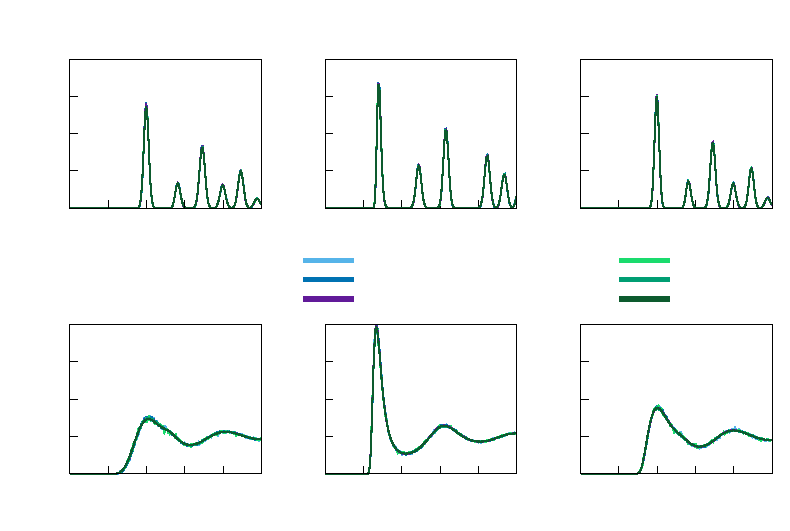
\includegraphics{ewald-vs-wolf}}%
    \gplfronttext
  \end{picture}%
\endgroup

    \caption{Radial distribution function for three pairs (from left to right
    \ce{Na-Na}, \ce{Na-Cl}, and \ce{Cl-Cl}) on two system: a solid NaCl crystal
    at \SI{300}{K} on top, and melted NaCl at \SI{2000}{K} on bottom.}
    % They are presented for two different softwares (LAMMPS and Domino), two
    % different electrostatic summation (Ewald and Wolf) and two simulation
    % methods (Monte Carlo or MC and molecular dynamics or MD).}
    \label{fig:ewald-vs-wolf:rdf}
\end{figure}

Another proof that my implementation is correct comes from the radial
distribution functions for all the simulation presented in
figure~\ref{fig:ewald-vs-wolf:rdf}. All simulations methods and electrostatic
summations gives the exact same curves, except for rounding errors and
statistical noise. This is also another evidence that Wolf summation is able to
reproduce properties predicted by Ewald summation.

In conclusion, Wolf summation seems to be able to replace Ewald summation, at
least for simple cases. It can also be twice as fast as Ewald, and simpler to
implement in simulation software. I did not have the time to use it in
conjunction with hybrid simulations, but this would be a natural extension of
this work.

\OnlyInSubfile{\printglobalbibliography}

\end{document}
